%!TEX root = main.tex
\section{Study Findings}
\subsection{Themes Emerging from Participatory Design\label{pd_findings}}
\begin{figure*}[ht!]
\centering
\vspace{-15pt}
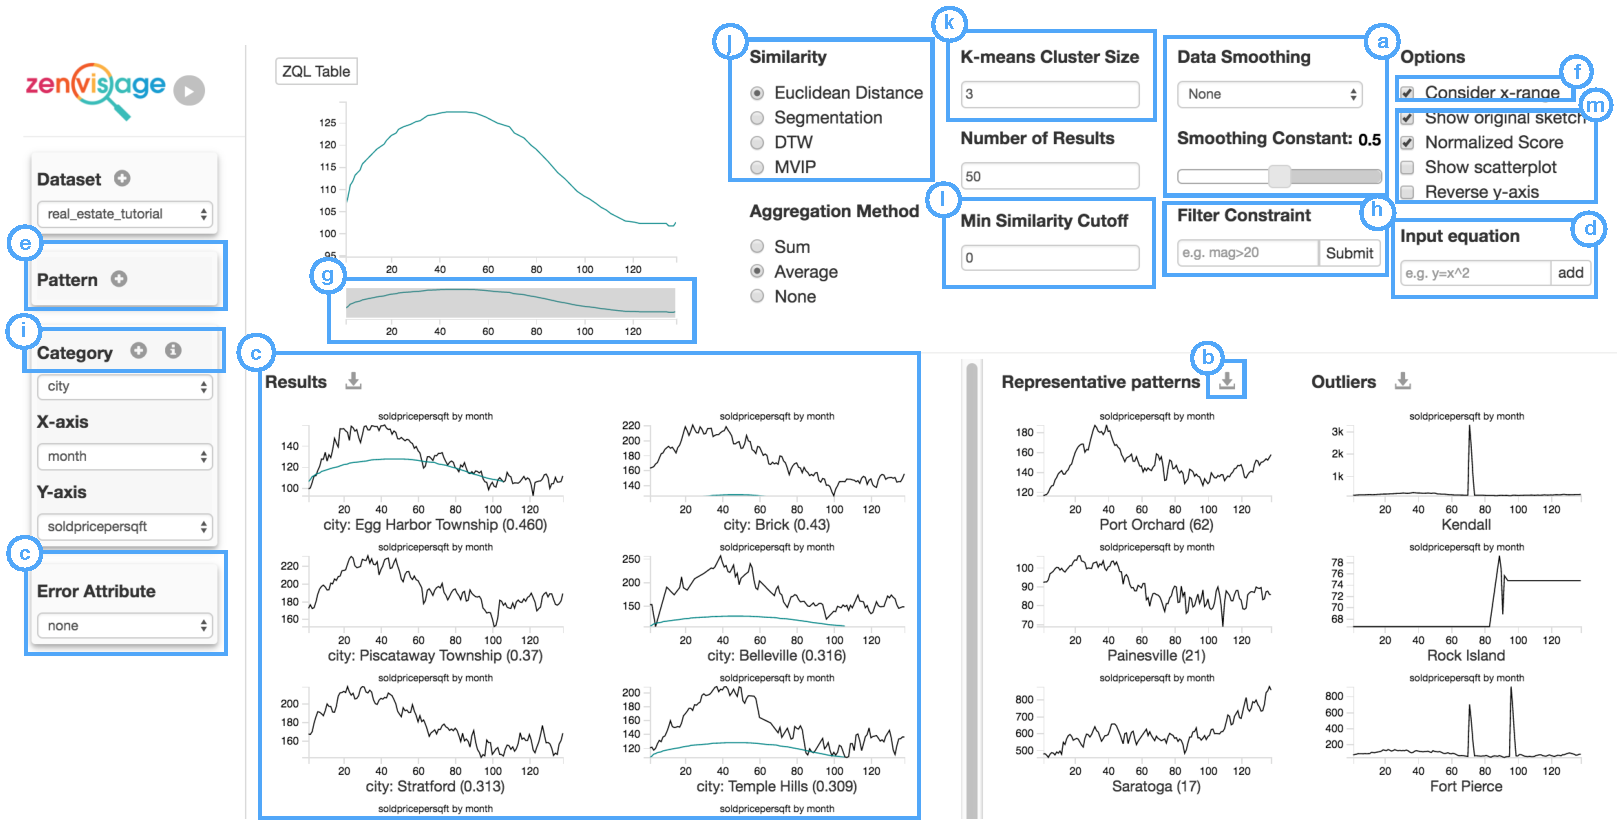
\includegraphics[width=\linewidth]{figures/newZV.pdf} %5.5
\vspace{-5pt}\caption{Our VQS after participatory design, which includes: the ability to preprocess via (a) interactive smoothing; (b, c) the ability to export data outputs ; querying functionalities via (d) equations and (e) patterns; query specification mechanisms including (f) x-range invariance, (g) x-range selection and filtering, (h) Filtering, and (i) Dynamic class creation; (j, k, l) system parameter options; (m) visualization display options. Prior to the participatory design, \zv only included a single sketch input with no additional options. \zv also displayed representative patterns and outlier patterns, as shown in Figure~\ref{oldZV}.}
\label{zvOverview}
\vspace{-14pt}
\end{figure*}

\par We employed participatory design with our scientists to incorporate key features missing in our original VQS, and unaddressed in their existing workflows. %We discovered three central themes encapsulating these features that are important to facilitate rapid hypothesis generation and insight discovery, but are missing in prior VQSs. While some of our findings echo prior work on system-level taxonomies of visualization tasks \cite{Amar2005,Heer2012}, we highlight how specific analytic tasks and interaction features could be used to enhance VQSs in particular. \techreport{In particular, we learned that \textit{participants wanted more control over the internals of the systems and an integrated workflow that helped streamline their analysis when using VQSs.}}
\subsection{Exact Shape Specification}
Most VQS has freehand sketching
mouse, pen,

sketching increasing trends

\stitle{Input Equations:} Our material science participants expressed that some solvents can have analytical models that characterize the relationships between chemical properties. They wanted to find solvents that satisfied these relationships. We implemented a feature that plots a given function (e.g. $y=x^2$) on the canvas, which is then used as input for similarity search (Figure \ref{zvOverview}d).

\subsection{Approximate Shape Specification}
While freehand sketching is intuitive mechanism for shape specification, a sketch query can be extremely imprecise, as pointed out by past works~\cite{correll2016semantics,Holz2009}. Many interfaces have developed constrained sketching mechanism, such as angular slope queries for specifying the slope of a trend line~\cite{Hochheiser2004} or decomposing a curve into piecewise straight querylines~\cite{ryall2005querylines}, to allow users to specify a `rough sketch' to convey the intent of an inexact match.  or varying level of tolerance deviation from sketched line. In \zv, we employ data smoothing to allow users to interactively change the degree of shape approximation they would like to apply to all data (and consequently the pattern matching). we developed an interface for users to interactively adjust the data smoothing algorithm and parameters on-the-fly to update the resulting visualizations accordingly (Figure \ref{zvOverview}a). Smoothing is also applied in Qetch~\cite{Mannino2018} for the same purpose. We originally included data smoothing since it was a common pre-processing step applied to the material science and astronomy use cases, as both had noisy and dense observational data. Both groups of participants noted that it was often hard to tell what the appropriate smoothing parameter should be applied simply by visualizing a small number of sampled visualization in an offline analysis. We found that the tight integration between smoothing and visual search additionally poses an interesting relationship between the smoothness of the curve and the degree of approximation for shape-matching in VQSs. If the visualization is over-smoothed, then shape matching would return results that only loosely resemble the query pattern. However, if no smoothing is applied, then the noise may dominate the overall trend, which could also lead to bad pattern matches.
%While the interactions in our original prototype enabled simple visual queries, many scientists were interested in extending their querying capabilities, either through different querying modalities or through more flexible query specification methods.

% While \zv does not attempt to solve all of the pre-processing issues that we faced during participatory design, we identified data smoothing as a common data cleaning procedure that could benefit from a tight integration between pre-processing and visual analysis. Data smoothing is a denoising procedure that generates a smoothed pattern approximating key features of the visualized trend with less noise.
\subsection{Range Selection}
\subsection{Flexible Matching}
the ability to change the choice of similarity metrics (Figure \ref{zvOverview}j) DTW and MVIP
\stitle{Consider/Ignore x-range:} We improved query specification by allowing users to change how the shape-matching criterion is applied. For finding supernovae, A1 primarily cared about the existence of a peak above a certain amplitude with an appropriate width of the curve, rather than the exact time that the event occurred, leading them to use the consider x-range feature. G1 also expressed that she does not really know what is the ``trigger point'' of when the expression level of a gene will rise and it would be interesting to find all ``rising'' profiles independent of the change-point.  We implemented an option to ignore the x-range in shape matching (Figure \ref{zvOverview}f) and a brushing mechanism that enables users to select the specific x-region they want to perform their shape matching on (Figure \ref{zvOverview}g).

\subsection{Filter Selection}
\par Past studies in taxonomies of visualization tasks have shown that it is important to design features that enable users to select relevant subsets of data in visual analytics\cite{Amar2005,Heer2012}. We designed two dynamic faceting features coupled with coordinated views that enabled users to specify subsets of data they are querying on and see immediate changes updated in the query, representative, and outlier results.

\stitle{Filtering Constraints:} Users with large datasets first used their domain knowledge to narrow down their search to a subset of data. This would increase their chances of finding an interesting pattern for a given query. To filter data, users could submit one or more SQL-like \texttt{WHERE} conditions as filter constraints in a text field (Figure \ref{zvOverview}h). \ccut{The filtering can be done on data columns associated with each pattern that is not visualized or on the visualized attributes.}
\subsection{Group Comparison}
\stitle{Dynamic Class Creation:} In order to address material scientists' needs for creating subsets (or classes) of data on-the-fly to make comparisons between them, we implemented dynamic class creation. This feature allows users to bucket data points into customized classes based on existing properties, and subsequently allows users to compare between the customized classes. For example, the scientists can create three different classes based on a single property alone: Solvents with ionization potential under -10 kJ/mol, over -8 kJ/mol, and ones that fall between -10 and -8 kJ/mol. Then, they could browse how the lithium solvation energy differed for the the three custom classes.
\npar Scientists can utilize multiple properties to create custom classes, effectively slicing-and-dicing the data based on their needs. The information regarding the created classes is displayed in the dynamic class information table or as a tooltip over the aggregated visualizations, as shown in Figure~\ref{dcc}.
\begin{figure}[h!]
\centering
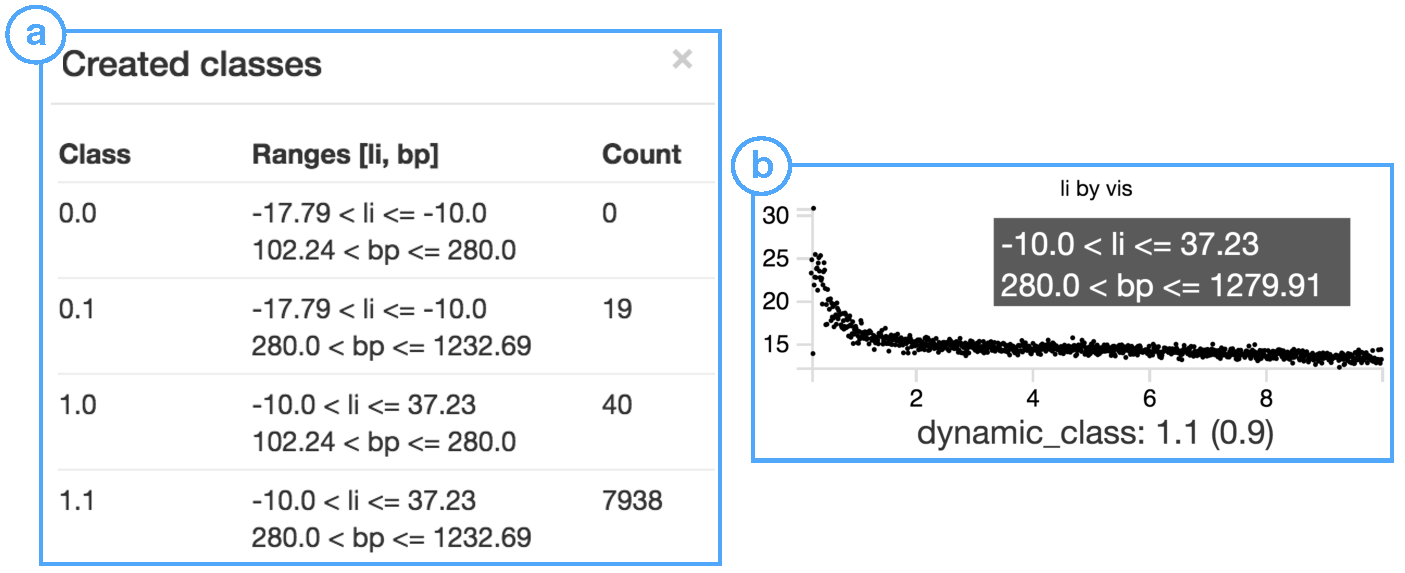
\includegraphics[width=\linewidth]{figures/dcc_example.pdf}
\vspace{-6pt}
\caption{Example of dynamic classes. (a) Four different classes with different Lithium solvation energies (li) and boiling point (bp) attributes based on user-defined data ranges. (b) Users can hover over the visualizations for each dynamic class to see the corresponding attribute ranges for each class. The visualizations of dynamic classes are aggregate across all the visualizations that lie in that class based on the user-selected aggregation method.}
\label{dcc}
\vspace{-10pt}
\end{figure}
\subsection{Concept querying}
\stitle{Upload Pattern as Query:} While the input equation is useful when simple analytical models exist, this may not be true for other domains. In these cases, users can upload a query pattern of a sequence of points (Figure \ref{zvOverview}e). This is useful for patterns generated from advanced computational models used for understanding scientific processes, usually as part of the downstream analysis of the exploratory workflow. %For example, the genetics team are trying to develop a time series prediction algorithm using machine learning based on some biological parameters \cite{Peng2016}. For the astronomy team, it is also common to compare synthetic light curves generated from simulations against observations \cite{Nugent1997}.
\subsection{Result-based querying}
- drag and drop
\subsection{Recommendation}
- representative and outliers

\subsection{Evaluation Study Results\label{eval_findings}}
We recorded audio, video screen captures, and click-stream logs of the participant's actions during the evaluation study. We analyzed the transcriptions of these recordings through open-coding and categorized every event in the user study. In addition, based on how each feature was used during the user study, we categorized the features into one of the three usage types:
\begin{denselist}
    \item Practical usage \textbf{[P]}: Features used in a sensible and meaningful way.
    \item Envisioned usage \textbf{[E]}: Features which could be used practically if the envisioned data was available or if they conducted downstream analysis, but was not performed due to the limited time during the user study.
    \item Not useful \textbf{[N]}: Features that are not useful or do not make sense for the participant's research question and dataset.
\end{denselist}
We chose to derive these labels from the user study transcription rather than through self-reporting to circumvent the bias that users may have when self-reporting, which can often artificially inflate the usefulness of the feature or tool under examination.
\begin{figure}[ht!]
    \centering
    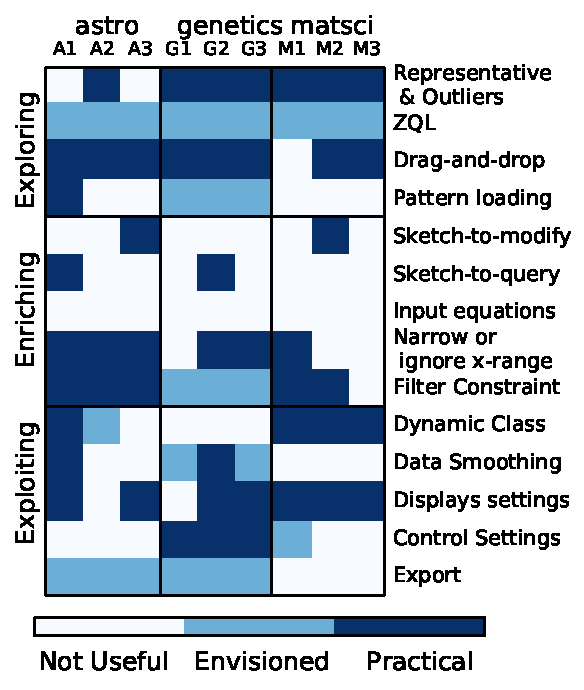
\includegraphics[width=0.7\columnwidth]{figures/result2.pdf}
    \vspace{-6pt}\caption{Heatmap of features categorized as practical usage (P), envisioned usage (E), and not useful (N). We find that participants preferred to query using bottom-up methods such as drag-and-drop over top-down approaches such as sketching or input equations. Participants found that data faceting via filter constraints and dynamic class creation were powerful ways to compare between subgroups or filtered subsets. The columns are arranged in the order of subject areas and the features are arranged in the order of the three foraging acts.}
    \label{feature_heatmap}
    \vspace{-5pt}
\end{figure}

\par The audio recordings and transcriptions of pre- and post-study interview questions are thematically encoded and summarized in Figure \ref{action_heatmap} and \ref{feature_heatmap}. Overall, we find that VQSs can enable rapid, fluid iteration, catalyzing new questions or insights; that different querying modalities in VQSs support different forms of exploration; and that expressive querying allowed participants to compose novel analysis patterns. In addition, we find that VQSs can be used for a range of tasks that go beyond just exploration; that participants used the outputs from VQSs in various ways; and that VQSs are most appropriate for certain types of datasets.
For the remaining paper, we will focus on developing a process model and design guideline for insight formation in VQSs and divert our thematic analysis of how VQSs fit into the context of an analysis workflow to our technical report.

% These observation inform our ----- search-browse paradigm
